%-*-coding: utf-8-*-
\FloatBarrier
\chapter{Описание алгоритма}

Основная идея заключается в составлении булевой формулы для набора входных деревьев и гибридизационного числа $h$, которая выполнима тогда и только тогда, когда существует гибридизационная сеть $N_h$ с гибридизационным числом $h$, отображающая все входные деревья.
Определив диапазон возможных значений гибридизационного числа, можно перебрать их все и составить формулы для фиксированных значений гибридизационного числа.
В итоге, ответом на задачу будет та из выполнимых формул, которая соответствует наименьшему гибридизационному числу.

\FloatBarrier
\section{Препроцессинг}

Перед тем как приступать к непосредственному кодированию булевой формулы, применяются несколько эвристик, позволяющих разбить задачу на подзадачи, и следовательно уменьшить ее сложность.
Для разбиения применяются следующие правила~\cite{bonet2009efficiently}:

\begin{enumerate}
	\item \textbf{Сокращение поддерева.} Если существует поддерево, содержащееся в каждом из исходных деревьев, значит в этой части эволюционной истории не наблюдалось ретикуляций, и для ее отображения достаточно древовидной структуры.
	Поэтому во всех исходных деревьях следует заменить это поддерево на лист с новой меткой.
	После решения задачи, в готовой сети, следует заменить этот лист на исходное поддерево.
	\item \textbf{Сокращение кластера.} Если существует кластер $A$, содержащийся в каждом из исходных деревьев, его также следует заменить на лист с новой меткой, а задачу построения минимальной гибридизационной сети решать для этого кластера отдельно.
	После решения задачи, следует заменить этот лист в готовой сети на сеть, являющуюся решением задачи для кластера $A$.
\end{enumerate}

Предложенный далее алгоритм предполагает, что у всех входных деревьев общий корень, но это предположение не выполняется для построенных подзадач.
Поэтому следует добавить фиктивный корень ко всем деревьям в каждой из подзадач.
Чтобы сохранить структуру деревьев корень добавляется вместе с новым фиктивным листом.
Этот процесс проиллюстрирован на Рис.~\ref{dummy-example}.
После решения задачи, фиктивный корень и фиктивный лист следует удалить.

\begin{figure}[t]
  \centering{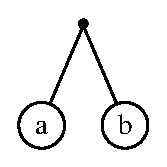
\includegraphics[width=2.6cm]{img/inp_dummy.eps}}
  \hspace{2cm}
  \centering{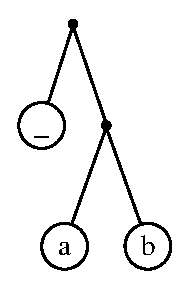
\includegraphics[width=3cm]{img/ans_dummy.eps}}
  \caption{Добавление фиктивного корня к дереву.}
  \label{dummy-example}
\end{figure}

\FloatBarrier
\section{Перебор гибридизационного числа}

Для решения задачи требуется найти такое минимальное $h$, что будет существовать гибридизационная сеть с гибридизационным числом равным $h$.
Существует несколько методик перебора значения $h$: последовательный перебор от больших значений к маленьким, от маленьких значений к большим и двоичный поиск.
В рамках данной работы были реализованы все три методики.
Если минимальное гибридизационное число равно $h_\mathrm{min}$, то, как правило, наибольшее количество вычислений потребуется для решения формулы при $h = h_\mathrm{min} - 1$.
Это обусловлено тем фактом, что найти какое-нибудь решение для солвера проще, чем, перебрав все варианты, убедиться, что решения не существует.
Экспериментальные результаты подтверждают это наблюдение, и поэтому перебор от маленьких значений к большим не представляет интереса, так как его производительность значительно ниже чем у остальных методов.
Результаты двоичного поиска практически повторяют результаты перебора от больших значений к маленьким, кроме случаев, в которых выполняется значительное количество проверок для значений меньших чем $h_\mathrm{min}$.


В данной работе используется перебор от больших значений к маленьким, как наиболее производительный метод.
Кроме того, было экспериментально обнаружено, что у многих из получаемых подзадач гибридизационное число мало, и времени на решение таких подзадач тратится мало, поэтому используется следующая эвристика: перед началом перебора производится попытка быстрого решения со значениями $h$ равными $0$, $1$, $2$ и $3$. В каждом из случаев солверу выделяется одна секунда на решение.


Объем вычислений можно очевидным образом сократить, если подобрать более точные границы возможных значений гибридизационного числа.
Существует несколько быстрых методов, основанных на различных эвристиках и методах линейного программирования, например PIRN$\mathrm{_{CH}}$~\cite{wu2010close}, RIATA-HGT~\cite{nakhleh2005riata} и MURPAR~\cite{park2012murpar}.

\FloatBarrier
\section{Кодирование булевой формулы}

Обозначим исходное множество деревьев за $T$, множество таксонов за $A$, размер $A$ за $n$, а предполагаемое гибридизационное число за $h$. Требуется построить булеву формулу, которая выполнима тогда и только тогда, когда существует сеть, с гибридизационным номером $h$, которая отображает все деревья из $T$.

Для начала, заметим, что исходные деревья содержат $2 n - 1$ вершин, а искомая сеть состоит из $2 (n + k) + 1$ вершин, т.к. добавляется фиктивный корень и фиктивный лист. Среди этих вершин $n + 1$ лист, $k$ ретикулярных вершин, и $n + k$ обычных вершин.

Введем нумерацию вершин по следующим правилам:

\begin{enumerate}
	\item Листья будут иметь номера в диапазоне $[0, n]$.
	\item Обычные вершины будут иметь номера в диапазоне $[n + 1, 2n + k]$.
	\item Ретикулярные вершины будут иметь номера в диапазоне $[2n + k + 1, 2(n + k)]$.
	\item Номер любого листа или обычной вершины меньше номера ее предка.
	\item У обычной вершины номер левого сына меньше номера правого сына.
	\item У ретикулярной вершины номер левого предка меньше номера правого предка.
\end{enumerate}

Кроме того, для каждой вершины $v$, введем следующие обозначения:

\begin{itemize}
	\item $\mathrm{PC}(v)$ --- множество возможных детей вершины $v$
	\item $\mathrm{PP}(v)$ --- множество возможных предков вершины $v$
	\item $\mathrm{PU}(v)$ --- множество вершин, которые могут находиться выше вершины $v$ в сети
\end{itemize}

А также обозначим множество листьев за $L$, множество ретикулярных вершин за $R$, а множество обычных вершин за $V$.

\FloatBarrier
\subsection{Кодирование структуры сети}
\label{sec:structure}

Чтобы закодировать структуру сети потребуются следующие переменные:

\begin{itemize}
	\item $l_{v,u}$ и $r_{v,u}$, где $v \in V, u \in PC(v)$. \\
	$l_{v,u}$ ($r_{v,u}$) истинно тогда и только тогда, когда вершина $u$ является левым (правым) ребенком вершины $v$.
	\item $p_{v,u}$, где $v \in L \cup V \backslash \{\rho\}, u \in PP(v)$. \\
	$p_{v,u}$ истинно тогда и только тогда, когда вершина $u$ является предком вершины $v$.
	\item $p^l_{v,u}$ и $p^r_{v,u}$, где $v \in R, u \in PP(v)$. \\
	$p^l_{v,u}$ ($p^r_{v,u}$) истинно тогда и только тогда, когда вершина $u$ является левым (правым) предком ретикулярной вершины $v$.
	\item $c_{v,u}$, где $v \in R, u \in PC(v)$. \\
	$c_{v,u}$ истинно тогда и только тогда, когда вершина $u$ является ребенком ретикулярной вершины $v$.
\end{itemize}

Всего требуется $O((n + k)^2)$ переменных. Заметив, что $k < n$, получаем оценку на количество переменных $O(n^2)$.

Необходимо закодировать уникальность каждой переменной, т.е. что у каждой вершины есть ровно один предок и ровно один левый и правый ребенок, и аналогичные утверждения для остальных переменных.
Для этого необходимо разбить утверждение вида <<ровно один>> на два утверждения <<хотя бы один>> и <<не более чем один>>.
В дальнейшем, для обозначения утверждения <<хотя бы один>> будет использоваться запись ALO, а для обозначения утверждения <<не более чем один>> будет использоваться запись AMO.

Утверждение ALO кодируется очевидным способом (на примере предков вершины $v$):
$$\mathrm{ALO}_p(v) = \bigvee\limits_{u \in PP(v)} p_{v,u}$$
Это утверждение означает, что одна из переменных, отвечающих за возможного предка вершины $v$ истинна.
Для остальных переменных утверждения <<хотя бы один>> записываются аналогичным образом.
Суммарно потребуется $O(n)$ утверждений ALO для всех переменных, где каждое из утверждений будет состоять из $O(n)$ переменных.
Общий размер формулы будет равен $O(n^2)$.

Утверждение AMO можно закодировать различными способами.
Самый простой способ --- попарное исключение (на примере предков вершины $v$):
$$\mathrm{AMO}_p(v) = \bigwedge\limits_{i, j \in PP(v)~:~i < j} \left(p_{v,i} \rightarrow \neg p_{v,j}\right)$$
Такой метод требует $O(n^2)$ утверждений для каждой переменной. 
Существуют более оптимальные кодирования.
В частности, в данной работе использовалось кодирование Bimander~\cite{nguyenefficient}, которое для каждой переменной требует $O(\mathrm{log}_2 n)$ дополнительных переменных, но позволяет сократить количество утверждений до $O(n \mathrm{log}_2 n)$.
Общий размер утверждений для кодирования AMO составит $O(n^2 \mathrm{log}_2 n)$.

Утверждения ALO и AMO для различных переменных указаны в секциях 1--4 Таблицы~\ref{network-table}.

\begin{table}[t]
\centering
\caption{Утверждения для кодирования структуры сети.}
\begin{tabular}{l | l | l}
  & Утверждение & Диапазон \\

  \hline
  1.1 &
  $\mathrm{ALO}_p(v)$ &
  \multirow{2}{*}{$v \in V; PP(v)$}
  \\
  1.2 &
  $\mathrm{AMO}_p(v)$ &
%  $v \in V; PP(v)$
  \\

  \hline
  2.1 &
  $\mathrm{ALO}_l(v)$ &
  \multirow{2}{*}{$v \in V; PC(v)$}
  \\
  2.2 &
  $\mathrm{AMO}_l(v)$ &
%  $v \in V; u_1 \dots u_k \in PC(v)$
  \\
  \hdashline

  2.3 &
  $\mathrm{ALO}_r(v)$ &
  \multirow{2}{*}{$v \in V; PC(v)$}
  \\
  2.4 &
  $\mathrm{AMO}_r(v)$ &
%  $v \in V; u, w \in PC(v)$
  \\

  \hline
  3.1 &
  $\mathrm{ALO}_c(v)$ &
  \multirow{2}{*}{$v \in R; PC(v)$}
  \\
  3.2 &
  $\mathrm{AMO}_c(v)$ &
%  $v \in R; PC(v)$
  \\

  \hline
  4.1 &
  $\mathrm{ALO}_{p^l}(v)$ &
  \multirow{2}{*}{$v \in R; PP(v)$}
  \\
  4.2 &
  $\mathrm{ALO}_{p^r}(v)$ &
%  $v \in R; u_1 \dots u_k \in PP(v)$
  \\
  \hdashline
  4.3 &
  $\mathrm{AMO}_{p^l}(v)$ &
  \multirow{2}{*}{$v \in R; PP(v)$}
  \\
  4.4 &
  $\mathrm{AMO}_{p^r}(v)$ &
%  $v \in R; u, w \in PP(v)$
  \\

  \hline
  5.1 &
  $l_{v,u} \rightarrow \neg r_{v,w}$ &
  $v \in V; u, w \in PC(v): u \geq w$
  \\
  5.2 &
  $p^l_{v,u} \rightarrow \neg p^r_{v,w}$ &
  $v \in R; u, w \in PP(v) : u \geq w$
  \\

  \hline
  6.1 &
  $l_{v,u} \rightarrow p_{u,v}$ &
  \multirow{3}{*}{$v \in V; u \in V \cap PC(v)$}
  \\
  6.2 &
  $r_{v,u} \rightarrow p_{u,v}$ &
  %$v \in V; u \in V \cap PC(v)$
  \\
  6.3 &
  $p_{u,v} \rightarrow (l_{v,u} \vee r_{v,u})$ &
  %$v \in V; u \in V \cap PC(v)$
  \\

  \hline
  7.1 &
  $l_{v,u} \rightarrow (p^l_{u,v} \vee p^r_{u,v})$ &
  \multirow{4}{*}{$v \in V; u \in R \cap PC(v)$}
  \\
  7.2 &
  $r_{v,u} \rightarrow (p^l_{u,v} \vee p^r_{u,v})$ &
  %$v \in V; u \in R \cap PC(v)$
  \\
  7.3 &
  $p^l_{u,v} \rightarrow (l_{v,u} \vee r_{v,u})$ &
  %$v \in V; u \in R \cap PC(v)$
  \\
  7.4 &
  $p^r_{u,v} \rightarrow (l_{v,u} \vee r_{v,u})$ &
  %$v \in V; u \in R \cap PC(v)$
  \\

  \hline 
  8.1 &
  $c_{v,u} \rightarrow p_{u,v}$ &
  \multirow{2}{*}{$v \in R; u \in V \cap PC(v)$}
  \\
  8.2 &
  $p_{u,v} \rightarrow c_{v,u}$ &
  %$v \in R; u \in V \cap PC(v)$
  \\

  \hline
  9.1 &
  $c_{v,u} \rightarrow (p^l_{u,v} \vee p^r_{u,v})$ &
  \multirow{3}{*}{$v \in R; u \in R \cap PC(v)$}
  \\
  9.2 &
  $p^l_{u,v} \rightarrow c_{v,u}$ &
  %$v \in R; u \in R \cap PC(v)$
  \\
  9.3 &
  $p^r_{u,v} \rightarrow c_{v,u}$ &
  %$v \in R; u \in R \cap PC(v)$
  \\

  \hline
  10.1\quad &
  $c_{v,u} \rightarrow \neg p^l_{v,w}$ &
  \multirow{2}{*}{$v \in R; u \in PC(v); w \in PP(v): u \geq w$}
  \\
  10.2 &
  $c_{v,u} \rightarrow \neg p^r_{v,w}$ &
  %$v \in R; u \in PC(v); w \in PP(v): u \geq w$
  \\

\end{tabular}
\label{network-table}
\end{table}

Чтобы удовлетворить 5 и 6 правило нумерации вершин вводятся утверждения, запрещающие неправильную нумерацию детей обычных вершин и предков ретикулярных вершин.
Эти утверждения приведены в секции 5 Таблицы~\ref{network-table}.

Кроме единственности переменных необходимо связать переменные отвечающие за предков с переменными отвечающими за детей.
Это делается очевидным образом: если вершина $u$ является сыном вершины $v$, то вершина $v$ должна быть предком вершины $u$, и наоборот.
Утверждения, связывающие детей и предков разных типов вершин указаны в секциях 6--9 Таблицы~\ref{network-table}.

Чтобы удовлетворить 4 правило нумерации вершин, необходимо добавить утверждения, упорядочивающие ребенка ретикулярной вершины относительно предков ретикулярной вершины.
Эти утверждения указаны в секции 10 Таблицы~\ref{network-table}.

Наиболее затратные утверждения --- утверждения упорядочивающие детей и предков.
Эти утверждения состоят из $O(n^2)$ переменных для каждой вершины.
Суммарный размер всех введенных утверждений составляет $O(n^3)$.

\FloatBarrier
\subsection{Кодирование отображения вершин деревьев на вершины сети}
\label{sec:mapping}

Осталось позаботиться о том, чтобы сеть отображала все исходные деревья.
Для этого введем следующие переменные:

\begin{itemize}

\item $x_{t,v_t,v}$, где $t \in T, v_t \in V(t), v \in V$. \\
$x_{t,v_t,v}$ истинно тогда и только тогда, когда вершина $v$ соответствует вершине $v_t$ из дерева $t$, то есть переменные $x$ для каждого дерева $t$ являются инъективным отображением множества вершин этого дерева в множество вершин сети. Пример части такого отображения показан на Рис~\ref{mapping-example}.
Заметим, что листья всех деревьев биективно соответствуют листьям сети т.к. множество таксонов одинаково для всех деревьев и сети.
Поэтому, переменные $x$ для листьев не вводятся.

\item $d_{t,v}$, где $t \in T, v \in R$. \\
$d_{t,v}$ истинно тогда и только тогда, когда для отображения дерева $t$ требуется выбрать левого предка у ретикулярной вершины $v$.

\item $u^r_{t,v}$, где $t \in T, v \in R$. \\
$u^r_{t,v}$ истинно тогда и только тогда, когда ребро в ребенка ретикулярной вершины $v$ используется для отображения дерева $t$.
Если ребенок ретикулярной вершины $v$ тоже является ретикулярной вершиной, то у него может быть зафиксировано направление не совпадающее с направлением его предка $v$, и тогда, при отображении дерева $t$, вершина $v$, вместо стягивания в ребро, полностью удалится.

\item $u_{t,v}$, где $t \in T, v \in V$. \\
$u_{t,v}$ истинно тогда и только тогда, когда вершина $v$ используется для отображения дерева $t$.

\item $a_{t,v,u}$, где $t \in T, v \in V, u \in PU(v)$. \\
$a_{t,v,u}$ истинно тогда и только тогда, когда вершина $u$ является первой вершиной на пути от вершины $v$ к корню, которая используется для отображения дерева $t$.
Другими словами, вершина $u$ является предком для вершины $v$, при отображении дерева $t$.
Заметим, что вершина $v$ может не использоваться для отображения.
На Рис.~\ref{mapping-example} вершина $u$ является предком для всех вершин ниже нее, при отображении дерева $t$.

\end{itemize}

\begin{figure}[t]
  \centering
  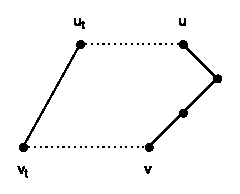
\includegraphics[width=5cm]{img/up_var.eps}
  \caption{Часть инъективного отображения вершин дерева (слева) на вершины сети (справа). Инъективное отображение изображено пунктирной линией. При отображении дерева, все ребра на пути от $u$ до $v$ стянутся в одно ребро, которое будет соответствовать ребру из $u_t$ в $v_t$.}
  \label{mapping-example}
\end{figure}

Введено $O(tn^2)$ новых переменных. Значит всего требуется $O(tn^2)$ переменных.

Для начала введем ALO и AMO утверждения для переменных $x$ и $a$, так как необходимо обеспечить их уникальность.
Заметим, что для переменных $x$ кроме утверждения <<не более чем одна вершина из сети соответствует вершине из дерева>> так же верное и утверждение <<не более чем одна вершина из дерева соответствует вершине из сети>>.
Эти утверждения указаны в секциях 1--2 Таблицы~\ref{mapping-table}.

\begin{table}[t]
\centering
\caption{Утверждения для кодирования отображения вершин деревьев на вершины сети.}
\begin{tabular}{l | l | l}
  & Утверждение & Диапазон \\

  \hline
  1.1 &
  $\mathrm{ALO}_{a_t}(v)$ &
  \multirow{2}{*}{$t \in T; v \in V \cup L \cup R; PU(v)$}
  \\
  1.2 &
  $\mathrm{AMO}_{a_t}(v)$ &
%  $t \in T; v \in V \cup L \cup R; PU(v)$
  \\

  \hline
  2.1 &
  $\mathrm{ALO}_{x_t}(v_t)$ &
  \multirow{2}{*}{$t \in T; v_t \in V(t); V$}
  \\
  2.2 &
  $\mathrm{AMO}_{x_t}(v_t)$ &
%  $t \in T; v_t \in V(t); V$
  \\
  \hdashline
  2.3 &
  $\mathrm{AMO}_{x_t}(v)$ &
  $t \in T; v \in V; V(t)$
  \\

  \hline
  3.1 &
  $x_{t,v_t,v} \rightarrow u_{t,v}$ &
  $t \in T; v \in V; v_t \in V(t)$  
  \\
  3.2 &
  $x_{t,\rho_t,\rho}$ &
  $t \in T; \rho_t = \rho(t)$
  \\

  \hline
  4.1 &
  $x_{t,u_t,u} \rightarrow a_{t,v,u}$ &
  \multirow{2}{*}{$t \in T; v \in L; u \in PP(v); u_t = p(v_t)$}
  \\
  4.2 &
  $a_{t,v,u} \rightarrow x_{t,u_t,u}$ &
%  $t \in T; v \in L; u \in PP(v); u_t = p(v_t)$
  \\
  \hdashline
  4.3 &
  $(x_{t,v_t,v} \wedge x_{t,u_t,u}) \rightarrow a_{t,v,u}$ &
  \multirow{2}{*}{$t \in T; v \in V; u \in PP(v); v_t \in V(t); u_t = p(v_t)$}
  \\
  4.4 &
  $(x_{t,v_t,v} \wedge a_{t,v,u}) \rightarrow x_{t,u_t,u}$ &
%  $t \in T; v \in V; u \in PP(v); v_t \in V(t): u_t = p(v_t)$
  \\
  \hdashline
  4.5 &
  $x_{t,v_t,v} \rightarrow \neg x_{t,u_t,u}$ &
  $t \in T; v \in V; u \in V; v_t \in V(t); u_t = p(v_t): u < v$
  \\

  \hline
  5.1 &
  $\neg x_{t,v_t,v}$ &
  $t \in T; v \in V; v_t \in V(t): v_t < \mathrm{size}(\mathrm{subtree}(v_t))$
  \\

  5.2 &
  $\neg x_{t,v_t,v}$ &
  $t \in T; v \in V; v_t \in V(t): v_t > \mathrm{size}(t) - \mathrm{depth}(v_t)$
  \\

  5.3 &
  $\neg x_{t,v_t,v} \vee \neg x_{t',v_{t'},v}$ &
  $t, t' \in T; v \in V; v_t \in V(t); v_{t'} \in V(t') :$
  \\
  & & \quad множества таксонов в поддеревьях $v_t$ и $v_{t'}$ не пересекаются

\end{tabular}
\label{mapping-table}
\end{table}

Благодаря фиктивным корням, известно, что корень сети $\rho$ соответствует корням каждого из деревьев, то есть для любого $t$ утверждение $x_{t,\rho_t,\rho}$ истинно.
Кроме того, очевидно, что если вершина $v$ соответствует какой-то вершине $v_t$ в дереве $t$, то вершина $v$ используется для отображения дерева $t$, то есть истинно утверждение $x_{t,v_t,v} \rightarrow u_{t,v}$.
Переменные $u$ введены для уменьшения размера формул, указанных в следующей секции.
Эти утверждения указаны в секции 3 Таблицы~\ref{mapping-table}.

Переменные $x$ и $a$ связаны следующим образом: если известно, что вершина $v$ из сети соответствует вершине $v_t$ из дерева $t$, а предку вершины $v_t$, вершине $u_t$, соответствует вершина $u$, то вершина $u$ является предком вершины $v$ при отображении дерева $t$.
И наоборот, если известно соответствие вершин $v$ и $v_t$, и известно, что вершина $u$ является предком вершины $v$ при отображении дерева $t$, то вершина $u$ должна соответствовать предку вершины $v_t$ в дереве $t$.
Заметим, что для листов не требуется явно указывать соответствие нижних вершин, так как они неявно подразумеваются.
Кроме того, чтобы удовлетворялось 4 правило нумерации, необходимо чтобы локальный порядок нумерации предков в деревьях сохранялся и в сети.
Другими словами, не допускается, чтобы вершина $u$ с меньшим номером соответствовала предку, а вершина $v$ с большим номером соответствовала сыну.
Эти утверждения приведены в секции 4 Таблицы~\ref{mapping-table}.

Также используются следующие эвристические ограничения, относящиеся к структуре деревьев:

\begin{itemize}
	\item номер вершины $v$ не может быть меньше, чем количество вершин в ее поддереве.
	\item номер вершины $v$ не может быть больше чем номер корня минус глубина вершины $v$.
	\item если поддеревья вершины $v_t$ и вершины $v_{t'}$ из деревьев $t$ и $t'$ соответственно содержат не пересекающиеся множества таксонов, то эти вершины не могут соответствовать одной и той же вершине $v$ из сети.
\end{itemize}

Эти утверждения приведены в секции 5 Таблицы~\ref{mapping-table}.

Наиболее затратными утверждениями являются утверждения, связывающие переменные $x$ и $a$.
Эти утверждения состоят из $O(n^2)$ переменных для каждой вершины и каждого дерева.
Суммарный размер всех введенных утверждений составляет $O(tn^3)$.

\FloatBarrier
\subsection{Кодирование трансляции связей <<предок--ребенок>> деревьев в сеть}
\label{sec:parent-child}

Необходимо отобразить явные связи <<предок-ребенок>> в деревьях на сеть.
Рассмотрим вершину сети $v$ и ее предка вершину $u$.
Если известно, что вершина $u$ используется для отображения дерева $t$, то вершина $u$ является предком вершины $v$, при отображении дерева $t$.
И наоборот, если известно что вершина $u$ является предком вершины $v$, при отображении дерева $t$, то вершина $u$ используется для отображения дерева $t$.
Если известно, что вершина $u$ не используется для отображения дерева, то вершины $u$ и $v$ имеют одного и того же предка, при отображении дерева $t$.
Это можно выразить следующим образом: если известно, что вершина $w$ является предком $u$, при отображении дерева $t$, то вершина $w$ является так же и предком $v$, при отображении дерева $t$.
И наоборот, если известно, что вершина $w$ является предком $v$ при отображении дерева $t$, то вершина $w$ является так же и предком $u$, при отображении дерева $t$.
Эти утверждения указаны в секции 1 Таблицы~\ref{child-parent-table}.

\begin{table}[t]
\centering
\caption{Утверждения для трансляции отношений <<предок--ребенок>> исходных деревьев в сеть.}
\begin{tabular}{l | l | l}
  & Утверждение & Диапазон \\

  \hline
  1.1 &
  $(p_{v,u} \wedge u_{t,u}) \rightarrow a_{t,v,u}$ &
  \multirow{2}{*}{$t \in T; v \in V \cup L; u \in V \cap PP(v)$}
  \\
  1.2 &
  $(p_{v,u} \wedge a_{t,v,u}) \rightarrow u_{t,u}$  &
  %$t \in T; v \in V \cup L; u \in V \cap PP(v)$
  \\
  \hdashline 
  1.3 &
  $(p_{v,u} \wedge \neg u_{t,u} \wedge a_{t,u,w}) \rightarrow a_{t,v,w}$ &
  \multirow{2}{*}{$t \in T; v \in V \cup L; u \in V \cap PP(v); w \in PP(u)$}
  \\
  1.4 &
  $(p_{v,u} \wedge \neg u_{t,u} \wedge a_{t,v,w}) \rightarrow a_{t,u,w}$ &
  %$t \in T; v \in V \cup L; u \in V \cap PP(v); w \in PP(u)$
  \\

  \hline
  2.1 &
  $(p^l_{v,u} \wedge d_{t,v} \wedge a_{t,u,w}) \rightarrow a_{t,v,w}$ &
  \multirow{4}{*}{$t \in T; v \in R; u \in R \cap PP(v); w \in PU(u)$}
  \\
  2.2 &
  $(p^l_{v,u} \wedge d_{t,v} \wedge a_{t,v,w}) \rightarrow a_{t,u,w}$ &
  %$t \in T; v \in R; u \in R \cap PP(v); w \in PU(u)$
  \\
  2.3 &
  $(p^r_{v,u} \wedge \neg d_{t,v} \wedge a_{t,u,w}) \rightarrow a_{t,v,w}$ &
  %$t \in T; v \in R; u \in R \cap PP(v); w \in PU(u)$
  \\
  2.4 &
  $(p^r_{v,u} \wedge \neg d_{t,v} \wedge a_{t,v,w}) \rightarrow a_{t,u,w}$ &
  %$t \in T; v \in R; u \in R \cap PP(v); w \in PU(u)$
  \\
  \hdashline
  2.5 &
  $(p^l_{v,u} \wedge d_{t,v} \wedge u_{t,u}) \rightarrow a_{t,v,u}$ &
  \multirow{2}{*}{$t \in T; v \in R; u \in V \cap PP(v)$}
  \\
  2.6 &
  $(p^r_{v,u} \wedge \neg d_{t,v} \wedge u_{t,u}) \rightarrow a_{t,v,u}$ &
  %$t \in T; v \in R; u \in V \cap PP(v)$
  \\
  \hdashline
  2.7 & 
  $(p^l_{v,u} \wedge d_{t,v} \wedge \neg u_{t,u} \wedge a_{t,u,w}) \rightarrow a_{t,v,w}$ &
  \multirow{4}{*}{$t \in T; v \in R; u \in V \cap PP(v); w \in PU(u)$}
  \\
  2.8 &
  $(p^l_{v,u} \wedge d_{t,v} \wedge \neg u_{t,u} \wedge a_{t,v,w}) \rightarrow a_{t,u,w}$ &
  %$t \in T; v \in R; u \in V \cap PP(v); w \in PU(u)$
  \\
  2.9 &
  $(p^r_{v,u} \wedge \neg d_{t,v} \wedge \neg u_{t,u} \wedge a_{t,u,w}) \rightarrow a_{t,v,w}$ &
  %$t \in T; v \in R; u \in V \cap PP(v); w \in PU(u)$
  \\
  2.10 &
  $(p^r_{v,u} \wedge \neg d_{t,v} \wedge \neg u_{t,u} \wedge a_{t,v,w}) \rightarrow a_{t,u,w}$ &
  %$t \in T; v \in R; u \in V \cap PP(v); w \in PU(u)$
  \\

  \hline
  3.1 &
  $(p^l_{v,u} \wedge \neg d_{t,v}) \rightarrow \neg u^r_{t,u}$ &
  \multirow{2}{*}{$t \in T; v \in R; u \in R \cap PP(v)$}
  \\
  3.2 &
  $(p^r_{v,u} \wedge d_{t,v}) \rightarrow \neg u^r_{t,u}$ &
  %$t \in T; v \in R; u \in R \cap PP(v)$
  \\
  \hdashline
  3.3 &
  $(p^l_{v,u} \wedge \neg d_{t,v}) \rightarrow \neg u_{t,u}$ &
  \multirow{2}{*}{$t \in T; v \in R; u \in V \cap PP(v)$}
  \\
  3.4 & 
  $(p^r_{v,u} \wedge d_{t,v}) \rightarrow \neg u_{t,u}$ &
  %$t \in T; v \in R; u \in V \cap PP(v)$
  \\

  \hline
  4.1 &
  $(p^l_{v,u} \wedge d_{t,v} \wedge u^r_{t,v}) \rightarrow u^r_{t,u}$ &
  \multirow{3}{*}{$t \in T; v \in R; u \in R \cap PP(v)$}
  \\
  4.2 &
  $(p^r_{v,u} \wedge \neg d_{t,v} \wedge u^r_{t,v}) \rightarrow u^r_{t,u}$ &
  %$t \in T; v \in R; u \in R \cap PP(v)$
  \\
  4.3 &
  $(c_{u,v} \wedge \neg u^r_{t,v}) \rightarrow \neg u^r_{t,u}$ &
  %$t \in T; v \in R; u \in R \cap PP(v)$
  \\
  \hdashline
  4.4 &
  $(p^l_{v,u} \wedge \neg u^r_{t,v}) \rightarrow \neg u_{t,u}$ &
  \multirow{2}{*}{$t \in T; v \in R; u \in V \cap PP(v)$}
  \\
  4.5 &
  $(p^r_{v,u} \wedge \neg u^r_{t,v}) \rightarrow \neg u_{t,u}$ &
%  $t \in T; v \in R; u \in V \cap PP(v)$
  \\
  \hdashline
  4.6 &
  $c_{v,u} \rightarrow u^r_{t,v}$ &
  $t \in T; v \in R; u \in \left(V \cup L\right) \cap PC(v)$
  \\

  \hline
  5.1 &
  $p_{v,u} \rightarrow \neg a_{t,u,w}$ &
  $t \in T; v \in V \cup L; u \in R \cap PP(v);$
  \\ & & \quad$w \in PU(u): w \leq v$
  \\
  5.2 &
  $(p_{v,u} \wedge a_{t,u,w}) \rightarrow a_{t,v,w}$ &
  $t \in T; v \in V \cup L; u \in R \cap PP(v);$
  \\ & & \quad$w \in PU(u): w > v$
  \\
  5.3 &
  $(p_{v,u} \wedge a_{t,v,w}) \rightarrow a_{t,u,w}$ &
  $t \in T; v \in V \cup L; u \in R \cap PP(v);$
  \\ & & \quad$w \in PU(u): w > v$
  \\

\end{tabular}
\label{child-parent-table}
\end{table}

Теперь рассмотрим ретикулярную вершину $v$ и ее предка $u$.

Если $u$ тоже является ретикулярной вершиной, и направление $u$ совпадает с выбранным направлением для дерева $t$, то вершины $v$ и $u$ имеют одного и того же предка, при отображении дерева $t$.
Это выражается аналогично предыдущему утверждению.
Если $u$ является обычной вершиной, ее направление совпадает с выбранным направлением для дерева $t$ и при этом используется для отображения дерева $t$, то вершина $u$ является предком вершины $v$ при отображении дерева $t$.
Если же вершина $u$ не используется, то вершины $v$ и $u$ имеют одного и того же предка, при отображении дерева $t$.
Эти утверждения указаны в секции 2 Таблицы~\ref{child-parent-table}.

Если выбранное направление для дерева $t$ не соответствует направлению $u$, то вершина $u$ не используется для отображения дерева $t$.
Соответствующие утверждения указаны в секции 3 Таблицы~\ref{child-parent-table}

Рассмотрим теперь связанные ретикулярные вершины, вершину--ребенка $v$ и вершину--предка $u$.
Если направление $u$ совпадает с направлением выбранным в вершине $v$, и $v$ используется для отображения дерева $t$, то $u$ тоже используется для отображения дерева $t$.
В случае, когда ретикулярная вершина $v$ не используется, то оба ее предка тоже не используются.
Если ребенок ретикулярной вершины $v$ является обычной вершиной, то вершина $v$ обязательно используется, так как нет другого способа попасть в ее ребенка.
Эти утверждения указаны в секции 4 Таблицы~\ref{child-parent-table}.

В секции 5 Таблицы~\ref{child-parent-table} указаны утверждения, отвечающие за корректность нумерации вершин для предков, при отображении дерева $t$.

Наиболее затратными утверждениями являются утверждения из секции 2 Таблицы~\ref{child-parent-table}.
Эти утверждения состоят из $O(n^2)$ переменных для каждой вершины и каждого дерева.
Суммарный размер всех введенных утверждений составляет $O(tn^3)$.

\FloatBarrier
\section{Решение булевой формулы и постпроцессинг}

Выбор подходящего солвера является темой для отдельного исследования. Некоторые эксперименты уже проводились~\cite{bonet2009efficiently}, и результаты отдельных солверов значительно превосходят результаты других. Не смотря на это, в рамках данной работы такие эксперименты не проводились. Для решения булевой формулы используется солвер CryptoMiniSat 4.2.0~\cite{cryptominisat}.

После того, как решена формула соответствующая минимальной гибридизационной сети, по полученным значениям переменных восстанавливается структура сети, удаляются фиктивный корень и фиктивный лист.
Затем, сети, полученные в результате решения подзадач, объединяются в одну сеть, являющуюся решением исходной задачи.
Итоговая сеть сохраняется в формате Graphviz~\cite{Gansner00anopen}.

\FloatBarrier
\section{Альтернативный способ кодирования структуры сети}

Предложенный способ кодирования структуры сети можно улучшить, если воспользоваться наблюдением, что можно последовательно добавлять в одно из исходных деревьев ретикулярную и обычную вершину, получая каждый раз корректную сеть.
Таким образом, проведя такую операцию $k$ раз, получится сеть с гибридизационным числом $k$.
После этого необходимо добавить утверждения из разделов~\ref{sec:mapping}~и~\ref{sec:parent-child}, связав с оставшиеся деревья с сетью.
Потенциальные плюсы такого подхода в том, что сеть задается меньшим количеством переменных и утверждений, что, в теории, позволит ускорить работу солвера.

Для начала условимся, что добавление ретикулярного события в дерево описывается следующим образом:

\begin{enumerate}
  \item Выбираются два ребра, которые будут подразбиты для вставки в них новых вершин.
  \item В одно из ребер вставляется обычная вершина, в другое вставляется ретикулярная вершина.
  \item Вторым предком новой ретикулярной вершины становится соответственно новая обычная вершина.
\end{enumerate}

Чтобы нумеровать ребра воспользуемся следующей схемой: рассмотрим обычную вершину $v$; ребро соединяющее вершину $v$ с ее предком будет иметь тот же номер, что и вершина $v$.
В случае ретикулярной вершины $u$, для описания ребер ведущих в предков понадобится два номера, поэтому номера ребер ведущих к предкам ретикулярной вершины $u$ будут иметь номера $2n - 1 + k + i$ и $2n + k + i$, если $u$ является $i$--й по порядку ретикулярной вершиной.

Для того, чтобы закодировать эти события, понадобятся следующие переменные:

\begin{itemize}
  \item $h_{v,e}$, где $v \in R, e \in E$. \\
  $h_{v,e}$ истинно тогда и только тогда, когда ретикулярная вершина $v$ вставлена в ребро $e$.
  \item $r_{v,e}$, где $v \in V, e \in E$. \\
  $r_{v,e}$ истинно тогда и только тогда, когда обычная вершина $v$ вставлена в ребро $e$.
\end{itemize}

Наиболее простой способ кодирования заключается в том, чтобы ввести следствие из новых утверждений, в утверждения, представленные в разделе~\ref{sec:structure}.
Такой подход не уменьшит общее количество утверждений, но позволит уменьшить количество реально значимых, независимых утверждений, что вместе с выбором подходящего солвера, позволит значительно ускорить перебор.

Для того, чтобы это осуществить, необходимо лишь указать, какие из переменных, отвечающих за предков будут истинны, после введения всех ретикулярных событий.

Для начала заметим, что нет никакого смысла добавлять одновременно и ретикулярную и обычную вершину в одно и то же ребро.
Кроме того, понадобятся уже известные ALO и AMO утверждения для того, чтобы обеспечить уникальность переменных $h$ и $r$.
Эти утверждения приведены в секции 1 Таблицы~\ref{second-enc-table}.

\begin{table}[t]
\centering
\caption{Утверждения для кодирования структуры сети.}
\begin{tabular}{l | l | l}
 & Утверждение & Диапазон \\

 \hline
 1.1 &
 $\neg h_{u_i, e} \vee \neg r_{v_i, e}$ &
 $v_i \in V; u_i \in R; e \in E$
 \\
 \hdashline
 1.2 &
 $\mathrm{ALO}_h(v)$ &
 \multirow{2}{*}{$v \in R; E(v)$}
 \\
 1.3 &
 $\mathrm{AMO}_h(v)$ &
%  $v \in R; E(v)$
 \\
 \hdashline
 1.4 &
 $\mathrm{ALO}_r(v)$ &
 \multirow{2}{*}{$v \in V; E(v)$}
 \\
 1.5 &
 $\mathrm{AMO}_r(v)$ &
%  $v \in V; E(v)$
 \\

 \hline
 2.1 &
 $(\neg h_{u_0, e} \wedge \neg r_{v_0, e} \dots \neg h_{u_k, e} \wedge \neg r_{v_k, e}) \rightarrow p_{v_e, u_e}$ &
 $u \in R; v \in V; e \in E; v_e \in e; u_e = p(v_e)$
 \\
 \hdashline
 2.2 &
 $\mathrm{LAST}_h(i, e) \rightarrow p_{v_e, u_i}$ &
 \multirow{2}{*}{$u \in R; v \in V; e \in E; v_e \in e$}
 \\
 2.3 &
 $\mathrm{LAST}_r(i, e) \rightarrow p_{v_e, v_i}$ &
% $u \in R; v \in V; e \in E; v_e \in e$
 \\

 \hline
 3.1 &
 $\mathrm{LAST}_h(i, e) \rightarrow (lp_{u_i, u_e} \vee lp_{u_i, v_i})$ &
 \multirow{2}{*}{$u \in R; v \in V; e \in E; u_e \in e$}
 \\
 3.2 &
 $\mathrm{LAST}_h(i, e) \rightarrow (rp_{u_i, u_e} \vee rp_{u_i, v_i})$ &
% $u \in R; v \in V; e \in E; u_e \in e$
 \\
 \hdashline
 3.3 &
 $\mathrm{LAST}_h(i, e) \rightarrow lp_{u_e, u_i}$ &
 $u \in R; e \in E; u_e \in e:$
 \\
 3.4 &
 $\mathrm{LAST}_r(i, e) \rightarrow lp_{u_e, v_i}$ &
 $~~~e$ ведет в левого предка
 \\
 \hdashline
 3.5 &
 $\mathrm{LAST}_h(i, e) \rightarrow rp_{u_e, u_i}$ &
 $u \in R; e \in E; u_e \in e$
 \\
 3.6 &
 $\mathrm{LAST}_r(i, e) \rightarrow rp_{u_e, v_i}$ &
 $~~~e$ ведет в правого предка
 \\

\end{tabular}
\label{second-enc-table}
\end{table}

Для удобства, введем формулы, означающие, что вершина $u_i$ ($v_i$) была добавлена последней в ребро $e$:
$$\mathrm{LAST}_h(i, e) = h_{u_i, e} \wedge \neg h_{u_{i+1}, e} \wedge \neg r_{v_{i+1}, e} \dots \neg h_{u_k, e} \wedge \neg r_{v_k, e}$$
$$\mathrm{LAST}_r(i, e) = r_{v_i, e} \wedge \neg h_{u_{i+1}, e} \wedge \neg r_{v_{i+1}, e} \dots \neg h_{u_k, e} \wedge \neg r_{v_k, e}$$

Теперь рассмотрим обычную вершину $v$.
Если в ребро над этой вершиной не добавлялось никаких новых вершин, то ее предок не изменился и является ее предком в дереве.
Иначе, ее предком будет вершина, добавленная самой последней в ребро над ней.
Так как вершины добавляются в сеть в порядке возрастания, то достаточно утверждения, что на $i$--м шаге вершина была добавлена в ребро $e$, а на шагах $i+1, i+2, \dots , k$ в ребро $e$ ничего не было добавлено.
Эти утверждения приведены в секции 2 Таблицы~\ref{second-enc-table}.

Аналогично для ретикулярных вершин.
Если в ребра, ведущие в предков ретикулярной вершины $v$ ничего не было добавлено, то эти ребра ведут либо в обычную вершину добавленную на том же шаге, либо в сответствующего предка из дерева.
Иначе, соответствующим предком будет вершина, добавленная самой последней в соответствующее ребро.
Эти утверждения приведены в секции 3 Таблицы~\ref{second-enc-table}.

К сожалению, на практике эта модификация не принесла ожидаемого ускорения, поэтому результаты ее тестирования не приведены в следующей главе.
Возможно, подбор подходящего солвера принесет какие-то результаты.
Кроме того, возможен вариант сведения, не использующий утверждения из раздела~\ref{sec:structure}, кодирующий всю структуру сети только переменными предложенными в этой главе.
Этот вариант сведения будет исследован в дальнейшей работе.
